



\begin{frame}{Jagt for stødende hund (rough shooting)}
    
     \begin{columns}[T]
        \begin{column}{0.58\textwidth}
            \begin{itemize}
                \item \textbf{Aktiv} jagtform – hund med kort søg letter vildtet som typisk nedlægges i bagskud 
                \item Typisk solo eller få jægere
                \item Der anvendes glatløbet haglgevær til jagtformen
                \item Udbredt jagtform i DK - passer til små arealer
            \end{itemize}
        \end{column}
        
         \begin{column}{0.4\textwidth}
            \centering
            \vspace{0.5em}
            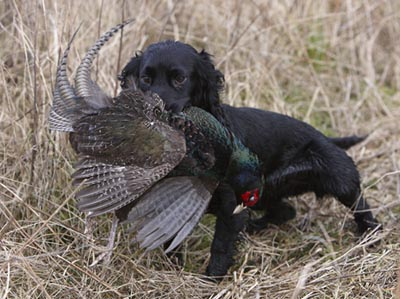
\includegraphics[width=\textwidth,height=0.82\textheight,keepaspectratio]
                {Billeder/Jagtformer/stoedende_01}
            % Alternativer – fjern kommentartegn hvis du vil skifte:
            % \includegraphics[width=\textwidth]{highseat-snow-forest-hunter.jpg}
            % \includegraphics[width=\textwidth]{hunter-highseat-morning-mist.jpg}
            % \includegraphics[width=\textwidth]{ansitz-jagttarn-skov.jpg}
        \end{column}
    \end{columns}
    
\end{frame}